\capitulo{REFERENCIAL TEÓRICO}

\secao{Problemas de Otimização}

Otimização é o processo de encontrar a melhor solução, também chamada de solução ótima para um determinado problema \cite{timoteo2005desenvolvimento}.\par

De acordo com \cite{steiglitz1982combinatorial} a constituição de um problema de otimização se deve aos termos vizinhança, ótimo local e ótimo global. O termo vizinhança trata de um subconjunto do conjunto de soluções do problema. Ótimo local pode ser tratado como o melhor resultado em uma vizinhança, e ótimo global é a melhor solução encontrada no conjunto de acordo com a função objetivo que é, uma especificação matemática, da relação entre as demais variáveis e a variável que desejamos maximizar ou minimizar.\par

Função objetivo é o objeto de nossa otimização. Pode ser um problema de otimização, um conjunto de teste para identificar os indivíduos mais aptos, ou mesmo uma "caixa preta" onde sabemos apenas o formato das entradas e a função nos retorna um valor que queremos otimizar. A grande vantagem dos algoritmos genéticos esta no fato de não precisarmos saber como funciona esta função objetivo, apenas tê-la disponível para ser aplicada aos indivíduos e comparar os resultados.

De acordo com a figura~\ref{fig:representacaoLocal}  pode se observar a relação entre ótimo local e ótimo global em conjunto de soluções de um problema típico de minimização, os quadrados mostram soluções quase ótimas chamadas de ótimo local e o circulo mostra a melhor solução encontrada dentro do conjunto de soluções, no caso o ótimo global.\par

\begin{figure}[!htb]
\caption[Representação de um problema de minimização com ótimos locais]{Representação de um problema de minimização com ótimos locais}
\label{fig:representacaoLocal}
\centering
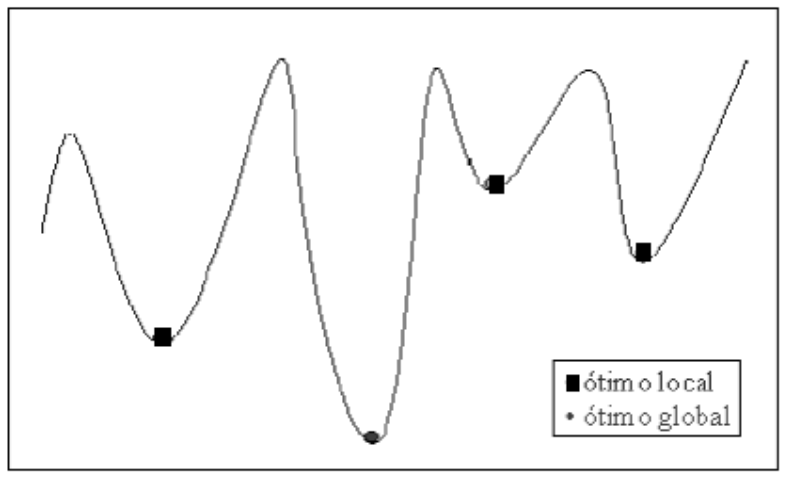
\includegraphics[scale=0.55]{imagens/problemaOtimizacao.png}
\\ \textbf{\footnotesize Fonte: \cite{timoteo2005desenvolvimento}}
\end{figure}
	
Segundo \cite{steiglitz1982combinatorial}, os problemas de otimização são divididos em duas categorias: problemas com variáveis contínuas e problemas com variáveis discretas. Problemas com variáveis discretas também podem ser conhecidos como Problemas de Otimização Combinatória (POC).\par

Conforme cita \cite{raupp2003introduccao}, o problema de otimização combinatória pode ser denominado como a ação de maximizar ou minimizar uma função objetiva de diversas variáveis sujeita a um conjunto de restrições, dentro de um contexto.\par

De acordo com \cite{opac-b1092847} problemas do tipo POC tratam do estudo matemático para encontrar agrupamentos, arranjos ou a seleção ótima de objetos discretos, logo, não permitindo, a utilização de métodos clássicos de otimização contínua para sua resolução.\par


Em seu trabalho \cite{golbarg2000otimizaccao} afirma que a ocorrência de problemas de otimização combinatória podem acontecer em diversas áreas, projetos de sistemas de distribuição de energia elétrica, posicionamento de satélites, roteamento ou escalonamento de veículos, sequenciamento de genes e DNA, classificação de plantas e animais.\par

De acordo com \cite{deleonardo} em problemas de otimização combinatória, cujo universo de dados é grande e existe um grande número de combinações, o que torna inviável a análise de todas soluções possíveis em um tempo adequado, utilizamos as heurísticas, também conhecidas como algoritmos heurísticos, que são métodos que compõem uma gama de soluções para problemas de otimização combinatória.

\secao{Heurística}

O termo heurística é derivado do grego \textit{heuriskein}, o que significa descobrir ou achar. De acordo com \cite{timoteo2005desenvolvimento} o significado da palavra em pesquisa operacional vai um pouco além da raiz etimológica. Segundo \cite{steiglitz1982combinatorial}, heurísticas são consideradas métodos de aproximação ou métodos de busca de solução. Deve se levar em consideração que não exista uma garantia formal de seu desempenho e uma garantia de que estas heurísticas que irão encontrar uma solução. As heurísticas, apesar de não garantirem encontrar a solução ótima para um problema, procuram por soluções consideradas de boa qualidade em um tempo computacional razoável.\par

Segundo \cite{evans1992optimization} heurísticas são necessárias para implementação de problemas NP Difícil, caso deseje-se resolver tais problemas em um tempo  razoável.\par

Ressalta-se que dentre as heurísticas, as chamadas meta-heurísticas, merecem especial atenção pois adotam técnicas para amenizar, a dificuldade que os métodos heurísticos têm de escapar dos ótimos locais. As meta-heurísticas podem partir em busca de regiões mais promissoras no espaço de soluções, alem disto, as meta-heurísticas possuem grande abrangência, podendo ser aplicada à maioria dos problemas de otimização combinatória \cite{nascimento2005aplicaccao}.\par

As meta-heurísticas surgiram como uma alternativa para amenizar a dificuldade que os métodos heurísticos tem de escapar dos chamados ótimos locais \cite{nascimento2005aplicaccao}.

Segundo \cite{adrianocesar} uma heurística é a instanciação de uma meta-heurística, ou seja, a aplicação da mesma em um problema específico de otimização.\par

Como exemplos de meta-heurísticas temos Busca Tabu (\textit{Tabu Search}), Otimização por Colônias de Formigas (\textit{Ant Colony Optimization}), Recozimento Simulado (\textit{Simulated Annealing}) e Algoritmo Genético (\textit{Genetic Algorithm}).\par

\subsecao{Busca Tabu}

Busca tabu (BT) é uma meta-heurística adaptativa, que utiliza uma estrutura de memória através de uma lista, contendo um histórico de evolução para evitar que o processo de busca forme ciclos, ou seja, o retorno a um ótimo local previamente visitado \cite{souza2000} , \cite{armentanointroduccao} e \cite{subramanian2006aplicaccao}.\par


Segundo \cite{subramanian2006aplicaccao} BT foi desenvolvida por \cite{glover1986future} com o objetivo de encontrar soluções para problemas de programação linear. Ao formalizar a técnica, o autor publicou uma série de trabalhos envolvendo diversas aplicações da meta-heurística. \par

Basicamente o funcionamento do BT a feito partir da definição de uma população inicial ${S_0}$, o algoritmo explora cada iteração de um subconjunto V da vizinhança N(S) da solução corrente S. O membro S’ de V com melhor valor nessa região segundo a função f(.) torna-se a nova solução corrente mesmo que S’ seja pior que S isto é, que f(S’) $>$ f(S) para um problema de minimização\cite{souza2000}. A figura~\ref{fig:buscaTabu} que se encontra no apêndice representa o pseudocódigo do algoritmo da Busca Tabu.

Segundo \cite{armentanointroduccao}  o algoritmo tem um intensivo uso de memória o que é uma característica essencial deste método. Para os autores o uso da memória pode ajudar a intensificar a busca em regiões com grande chances de se encontrar o resultado, ou até mesmo, diversificar a busca através de regiões inexploradas.

Ainda de acordo com \cite{armentanointroduccao}  devemos adotar alguns procedimentos para que o processo de busca tenha um melhor resultado: listas tabu dinâmicas, passagens por regiões planas, intensificação, diversificação, \textit{path relinking}. Listas tabu dinâmicas tem como objetivo evitar que o algoritmo entre em processo de ciclo. Passagens por regiões planas pode levar o algoritmo a pensar que não existem melhoras significativas na qualidade das soluções e atingir o critério de parada. Para evitar esta situação é necessário aumentar o tamanho da lista tabu enquanto o algoritmo estiver passando pela região plana e voltar a reduzir quando houver mudança no valor da função objetiva. Intensificação são técnicas utilizadas para concentrar os esforços da pesquisa em regiões consideradas promissoras. Diversificação é uma técnica que utiliza memória de longo prazo para redirecionar a pesquisa para regiões que ainda não foram suficientemente exploradas. PathRelinking trada da intensificação de incorporar atributos de soluções de boa qualidade (chamadas de soluções elite), em seguida explora caminhos que contenham uma ou mais soluções de elite.

Ainda segundo \cite{armentanointroduccao} uma característica importante do método é que a solução final tem pouca ou nenhuma dependência da escolha feita para a solução inicial, isso graças aos mecanismos implementados pelo método, que fogem de ótimos locais.

\subsecao{Recozimento Simulado}

Recozimento Simulado é a técnica de busca local probabilística, proposta originalmente por \cite{kirkpatrick1983optimization}, que se fundamenta em uma analogia com a termodinâmica, ao simular o 
resfriamento de um conjunto de átomos aquecidos.\par 

Isto é, conforme \cite{noronha2003abordagem} em analogia a física da matéria: levando um cristal a sua temperatura de fusão, as moléculas estão desordenadas e se agitam livremente. Ao resfriar-se a amostra de maneira infinitamente lenta, as moléculas vão adquirir a estrutura cristalina estável que tem um nível de energia mais baixo possível.\par 

Segundo \cite{souza2002experiencias} o processo se inicia com um membro qualquer do espaço de soluções, normalmente gerado aleatoriamente, e seleciona um de seus vizinhos randomicamente. Se este vizinho for melhor que o original ele é aceito e substitui a solução corrente. Se ele for pior por uma quantidade ∆, ele é aceito com uma probabilidade e -∆/T , onde T decresce gradualmente conforme o progresso do algoritmo. Esse processo é repetido até que T seja tão pequeno que mais nenhum movimento seja aceito. A melhor solução encontrada durante a busca é tomada como uma boa aproximação para a solução ótima. Originalmente, \textit{Simulated Annealing} foi derivado de simulações em termodinâmica e por esta razão o parâmetro T é referenciado como temperatura e a maneira pela qual ela é reduzida é chamada de processo de resfriamento.


A figura~\ref{fig:resozimentoSimulado} que se encontra no apêndice representa o pseudocódigo do algoritmo \textit{Simulated Annealing}.

Conforme \cite{aarts1988simulated} a analogia com a otimização (combinatória ou não) é bastante direta. Os estados da matéria são as soluções realizáveis, a quantidade objetiva substitui a energia, os estados metaestáveis da matéria sendo ótimos locais e a estrutura cristalina corresponde ao ótimo global.\par 

\subsecao{Algoritmos genéticos}

%o que é 
De acordo com \cite{goldberg1989genetic} Algoritmos Genéticos (AG) são baseados na teoria da evolução das espécies elaborada por \cite{darwin1968origin} utilizando os conceitos da biológia tais como genes, individuo, população, cromossomos, cruzamento, mutação e seleção. Estes algoritmos foram introduzidos por \cite{holland1975adaptation} para resolver os problemas chamados \textit{timetabling}.

Para entender melhor \cite{mitchell1998introduction} descreve os principais termos biológicos necessários para o funcionamento dos algoritmos genéticos. Gene se trada de uma característica particular de um cromossomo. Um cromossomo é composto por um ou mais genes, pode se dizer também que é uma sequencia de genes que será caracterizada como a solução do problema. \textit{Fitness} significa a aptidão do indivíduo em um determinado ambiente. Individuo é a combinação do cromossomo mais o \textit{fitness} calculado através da função objetiva. População é um grupo de indivíduos. Geração se trata de cada interação do algoritmo.\par

Em seu trabalho \cite{lucas2000algoritmos} descreve algoritmos genéticos da seguinte forma. São algoritmos que trabalham sobre uma população, através de uma função de adaptação, para que aconteça a evolução. Primeiramente é inicializada uma população, logo após iram acontecer os processos de seleção, reprodução também conhecida como \textit{crossover} e mutação, os mesmos ocorreram a cada geração até que os critérios de parada aconteçam. Também afirma que os termos utilizados pertencem à tradição existente no meio da computação evolutiva de utilizar, com certa liberdade os termos da biologia.

Segundo \cite{oliveira2005algoritmo}, o processo de evolução executado por um algoritmo genético corresponde a um procedimento de busca no espaço de soluções potenciais para o problema e, como enfatiza \cite{michalewicz1996evolutionary}, esta busca requer um equilíbrio entre dois objetivos aparentemente conflitantes: a procura das melhores soluções na região que se apresenta promissora ou fase de intensificação e a procura de outra região ou exploração do espaço de busca, também conhecida como diversificação.\par

\begin{figure}[!htb]
\caption[Estrutura funcional de um algoritmo genético típico]{Estrutura funcional de um algoritmo genético típico}
\label{fig:ag}
\centering
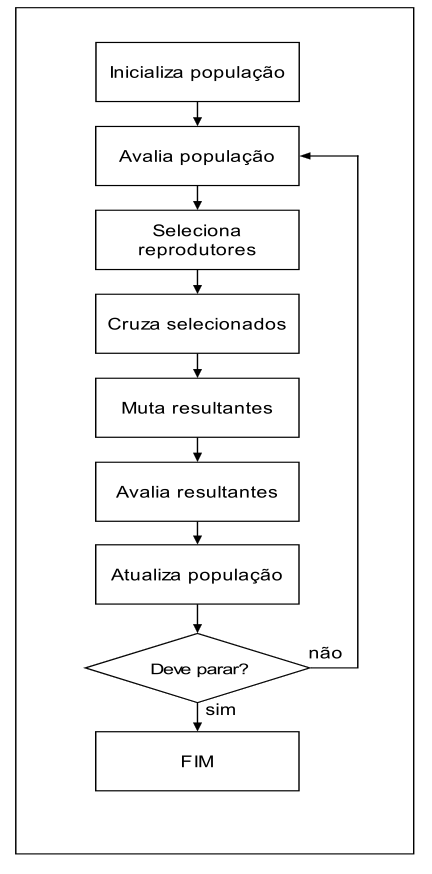
\includegraphics[scale=0.7]{imagens/ag.png}
\\ \textbf{\footnotesize Fonte: \cite{de1999introduccao}}
\end{figure}

%falar sobre população inicial

A Figura~\ref{fig:ag} trata de uma estrutura funcional típica de um algoritmo genético, \cite{de1999introduccao} cita em seu trabalho que o primeiro passo a ser tomado é a geração de uma população inicial, que é formada através de métodos aleatórios para gerar os indivíduos, assim teremos uma biodiversidade na população. Durante o processo evolutivo todos indivíduos da população são avaliados e cada um deles recebe o seu \textit{fitness}, o que representa a qualidade da solução representada por ele.\par

%falar sobre seleção

Segundo \cite{lobo2005soluccao} existem vários métodos para selecionar indivíduos para execução dos operadores genéticos, em seu trabalho o autor apresenta os seguintes métodos. Seleção por roleta é um método tradicional, para cada indivíduo é atribuído um espaço na roleta sendo o tamanho proporcional ao valor da aptidão do individuo. Esta roleta gira N vezes onde N é o numero do tamanho da população, selecionando assim os pais para próxima geração. Seleção por torneio são selecionados X indivíduos da população onde X é um valor aleatório anterior e escolhidos os dois que que contêm o maior valor de aptidão no caso os país, segundo o autor este método é o mais utilizado, pois oferece a vantagem de não exigir que a comparação seja feita entre todos os indivíduos da população.\par

%falar sobre operadores genéticos.

De acordo com \cite{goes2005otimizaccao} os principais operadores genéticos, utilizados ao se desenvolver algoritmos genéticos são inversão, mutação e \textit{crossover}, são responsáveis em realizar transformações nos indivíduos da população mas cada um possui suas diferentes funções dentro do algoritmo.\par
Inversão é um operador que modifica a genética de um gene ele é fundamental para garantir a biodiversidade da população, ainda segundo \cite{goes2005otimizaccao} o operador mutação  desenvolve o mesmo papel que o operador inversão, o mesmo cita que vários autores consideram inversão e mutação como o mesmo operador genético e também afirmam que são os operadores mais importantes e optam por trabalhar somente com estes operadores. Estes operadores são fundamentais para o desenvolvimento de algoritmos genéticos por evitarem a convergência prematura da solução, ou seja, quando uma população se estabiliza com uma adaptação pouco adequada, podemos dizer então que, um super-indivíduo domina o processo seletivo de tal forma que não é possível gerar filhos melhores, este mesmo super-indivíduo transmite suas características para toda a população.\par

O operador cruzamento também conhecido como \textit{crossover} é um operador genético onde é selecionado um ponto de corte produzindo duas cabeças e duas caldas após isto é realizada a troca das caldas dos pais criando dois filhos contendo material genético similares aos dos pais a figura~\ref{fig:pontoCorteAG} mostra onde é realizado o ponto de corte como ficam os filhos criado após a troca das caldas \cite{de1999introduccao}.

\begin{figure}[!htb]
\caption[Ponto de corte \textit{crossover}]{Ponto de corte \textit{crossover}}
\label{fig:pontoCorteAG}
\centering
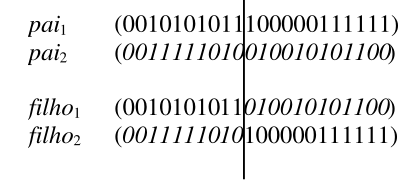
\includegraphics[scale=0.7]{imagens/crossoverAG.png}
\\ \textbf{\footnotesize Fonte: \cite{de1999introduccao}}
\end{figure}

No artigo apresentado pelos autores \cite{de1999introduccao} o elitismo é descrito como um operador genético que foi proposto por \cite{DeJong} em seu trabalho, que é dos pioneiros sobre algoritmos genéticos. Uma vez que os melhores indivíduos, de acordo com a função objetiva, podem ser perdidos entre uma geração e outra devido ao corte do \textit{crossover} e a execução da mutação, torna-se interessante transferir o melhor indivíduo para a próxima geração, o nome dado para está estratégia se chama elitismo uma técnica muito utilizada ao se desenvolver AGs. Os autores apresentam gráficos que mostram o desempenho da utilização do operador, segundo os mesmo quando se é utilizado o operador fica claramente observado que, com o uso do elitismo o algoritmo encontra a solução mais rápida, do que quando não ocorre a utilização do operador.

Segundo \cite{hamawaki2011geraccao} e \cite{oliveira2005algoritmo} algoritmos genéticos são eficientes para encontrar soluções ótimas ou quase ótimas, pois as limitações são minimas dos demais métodos de busca tradicionais. Ainda segundo \cite{oliveira2005algoritmo}, os algoritmos genéticos têm se mostrado ferramentas poderosas para resolver problemas onde o espaço de busca é muito grande e os métodos convencionais se mostraram ineficientes.\par


\secao{TimeTabling}

Segundo \cite{kripkasimulated} os problemas de programação de horários (PPH), também conhecidos como \textit{TimeTabling}, são os problemas que mais se destacam nas organizações acadêmicas. De acrodo com \cite{schaerf1999survey} estes problemas são divididos em três categorias \textit{school timetabling}, \textit{course timetabling} e \textit{examination timetabling}.\par

\textit{School TimeTabling}: Trata-se basicamente da geração de horários semanais, em escolas de segundo grau, onde deve-se evitar os choques entre os horários das disciplinas e que cada professor receba apenas uma turma para cada horário. Neste caso o aluno recebe um número fixo de disciplinas a serem cursadas.\par

\textit{Course TimeTabling}: Diz respeito à alocação de aulas de uma universidade típica. Neste problema os alunos podem escolher as matérias em que vão se matricular, portanto o problema tem como objetivo minimizar os possíveis choques entre as disciplinas, professores e horários disponibilizados pela instituição de ensino.\par

\textit{Examination TimeTabling}: Aborda o problema de programação de horários dos exames da instituição, de maneira que, disciplinas que tenham alunos em comum, distanciem o máximo possível as datas dos exames.\par

Segundo \cite{pinheiro2001ambiente} o problema de programação de horários vem sendo abordado desde a década de 60, sendo que os primeiros trabalhos a se destacarem foram realizados na década de 80.\par

O Problema de Alocação de Salas (PAS) também conhecido como \textit{Classroom Assignment} é tratado como parte do problema de programação de cursos universitários \textit{course timetabling}. Conforme cita \cite{marinho2005heuristicas} várias instituições universitárias se deparam com o PAS durante o início de cada semestre letivo. Este problema é considerado NP-Difícil por \cite{even1975complexity} e \cite{carter1992classroom}, com isto, a determinação da solução ótima do problema, em um período de tempo aceitável se torna uma tarefa difícil.\par

Uma vez que é de extrema dificuldade encontrar a solução ótima do PAS em tempo razoável, este problema é normalmente tratado através de técnicas heurísticas, que apesar de não garantirem encontrar a solução ótima do problema, são capazes de retornar uma solução de qualidade em um tempo adequado.\cite{nascimento2005aplicaccao}.Segundo \cite{even1975complexity} o PAS pertence a classe de Problemas de Otimização Combinatória (POC).\par

Segundo \cite{kripkasimulated} o problema deve considerar que as disciplinas dos cursos universitários já tenham seus horários de início e de término definidos. O problema se resume então na alocação das disciplinas às salas desta universidade respeitando os horários destas disciplinas e as demais restrições exigidas.

Em seu trabalho \cite{souza2000} afirma que boa parte das universidades ainda resolvem este problema de forma manual, o que torna o processo árduo e demorado, podendo levar vários dias para ser concluído.\par



\secao{Trabalhos Relacionados}

Foram encontrados vários trabalhos relacionados ao tema de resolução de problemas de otimização combinatória através de meta-heurísticas. Os trabalhos relacionados escolhidos contém formas diferentes de resolução do PAS.\par

Ao desenvolver seu trabalho \cite{subramanian2006aplicaccao} concluirão que o BT teve um resultado adequado e sempre produzindo melhorias durante o processo de refinamento da solução inicial, o mesmo também afirma que o algoritmo apresentou-se robusto, uma vez que não houve grande variação na solução final, portando o mesmo sempre gerava soluções satisfatórias.

A abordagem realizada por \cite{silva2005estudo} foi através da meta-heurística recozimento simulado. A autora afirma que o algoritmo se mostrou eficiente para resolução do PAS, produzindo bons resultados ao atender a maioria dos requisitos do problema, o uso deste algoritmo é indicado quando se trada da substituição do processo manual realizado pelas instituições de ensino.

O trabalho desenvolvido por \cite{hamawaki2011geraccao} é realizado através da utilização de algoritmos genéticos, segundo a autora a aplicação do AG e a analise dos resultados obtidos é possível concluir que as técnicas implementadas favorecem a obtenção de uma solução satisfatória e eficiente.

A resolução do problema PAS através de diferentes técnicas meta-heurísticas, podemos notar que a conclusão dos trabalhos apresentam uma solução satisfatória segundo ao autores ao se utilizar os estas técnicas através dos algoritmos.\par
